\section{Trust Management}
\label{sec:trust-management}
Trust is the reliance on the integrity or strength of a person or thing
\autocite{Dictionary2013} Trust can be sub-categorized as reputation
, and it plays a vital role in an organization \autocite{Liu2006}. In every organization, employee trust plays
a pivotal role and trust issues can make or break the culture of organization. There is a
lot stress involved in working in an environment where data is highly classified and trust
between the employees is minimal. Without trust, an organization will not meet its
quality standard. Hence, trust must exist for the organization to be successful.

\subsection{Data Transmission based on Trust}
Within CloudAssure, this module evaluates the trust metric \( Tr_{new} \) used
as an input to planning as described in Section \ref{sec:planning}. The transmission of data across various
nodes is done by evaluation of a metric called Trust Value. A \gls{sa} 
uses the trust values of the nodes as part of the planning phase (Section
\ref{sec:planning}). A Trust server publishes the trust value of each node to
the \gls{sa}. In this way, the document is transmitted between
nodes. The representation of transmission of a single document from Node A to Node B is
shown in the Figure ~\ref{fig:DataTransmission}.
\begin{figure}[h!]
    \begin{center}
        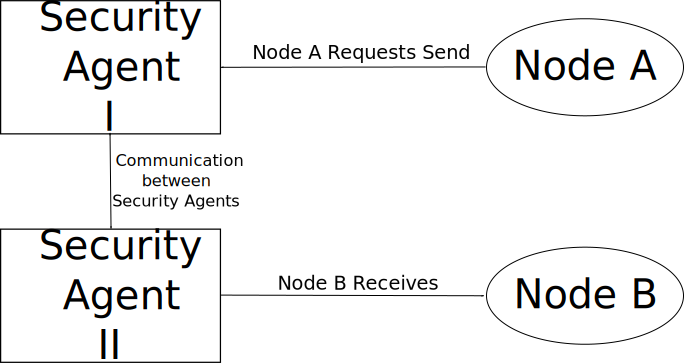
\includegraphics[width=0.90\textwidth]{Figures/DataPropagation.eps}
        \caption{Data Propagation}
        \label{fig:DataTransmission}
    \end{center}
\end{figure}


In Figure~\ref{fig:DataTransmission}, the classification of the document
is evaluated by \gls{sa} I as described in Section~\ref{sec:classification}. 
The \gls{sa} at level I, communicate the trust metric of the sender, as well as
the document classification with the \gls{sa} at level II. The Planning
component then takes over to build a localized graph of Node B. The planning
component will then recommend to the sender if the document should be sent to
Node B. The user is free to ignore this suggestion

Now, in an organization there are a number of employees working at various levels like
Chief Manager, Manager, Senior Associate, Associate, Junior etc. Based on this hierarchy we
have divided the group of nodes to be at each level and these groups of nodes are maintained
by a \gls{sa} (Figure~\ref{fig:TrustTransmission}. Now each \gls{sa} is connected to a number of nodes and all
the \Gls{sa} are linked together to a single trust server. The trust server
maintains trust values of every node, at every level. Because document transfer
requests occur asynchronously, the trust value of the respective node is updated
continuously. This allows the planning algorithm to
make the most informed decision possible. 



\begin{figure}[h!]
    \begin{center}
        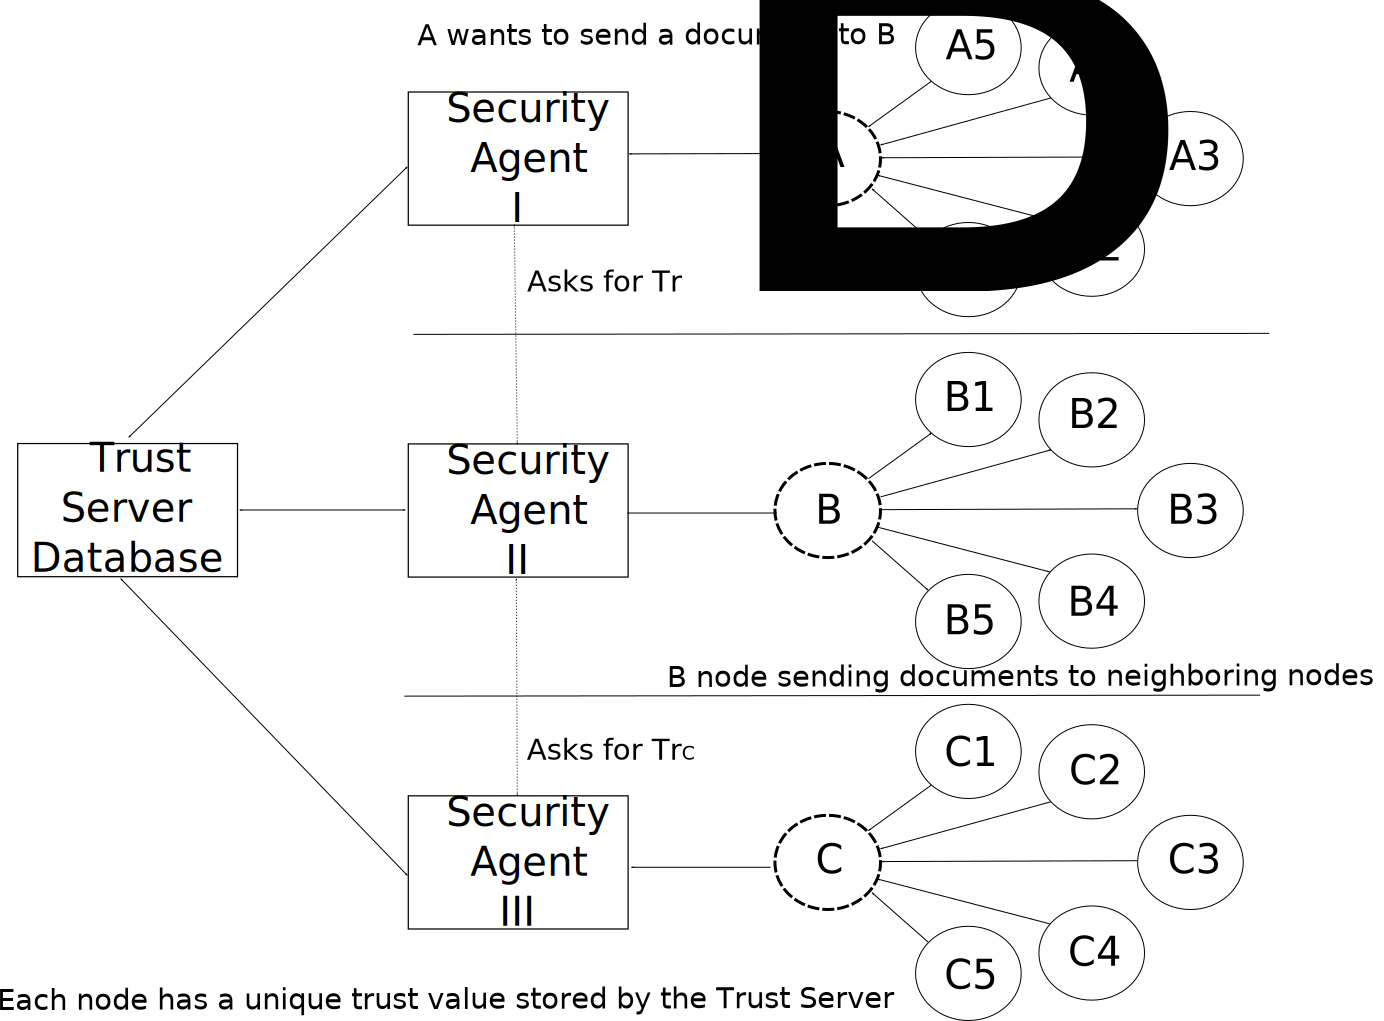
\includegraphics[width=0.90\textwidth]{Figures/TrustValuePropagation.eps}
        \caption{Trust Value Propagation}
        \label{fig:TrustTransmission}
    \end{center}
\end{figure}
\FloatBarrier

\subsection{Trust Values Criteria}
\label{sec:trust_value_criteria}
Now we see how trust is used, how is it managed?
Trust Value (\(Tr_{new}\)) incorporates the following high-level
criteria:
\begin{enumerate}
    \item A Node sends a highly sensitive document to another node. If the document leaks from
        the destination node, the receiver's trust value is reduced by a high value.
    \item A Node sends a lowly sensitive document to anther node. If the document leaks, as
        before, the receiver's trust value is reduced by a lower value.
\end{enumerate}

To achieve these high-level criteria, we use the following metrics:
\begin{enumerate}
    \item The \emph{Classification} of the document to be sent.
    \item The \emph{Similarity} of the document compared to past received
        documents.
    \item The \emph{old trust value} (\(Tr_{old}\)).
    \item The \emph{total number of documents} shared by a particular node.
\end{enumerate}

\subsection{Trust Value Equation}
Based on the above factors, CloudAssure uses a trust value equation to planning 
decisions. Similar to classification, our initial trust evaluation equation
turned out to be ineffective. Firstly, we will discuss the failed attempt
(Section~\ref{sec:initial_trust_equation}), followed by our recommended equation
(Section~\ref{sec:recommended_trust_equation}). 

\subsubsection{Initial Trust Equation}
\label{sec:initial_trust_equation}
The trust value is calculated based on the factors described in
Section~\ref{sec:trust_value_criteria}. This first equation attempted to combine
the localized graph concepts. This
proved to be ineffective and was later moved into the planning component. The
artifact of this decision is in the node notation of
Equation~\ref{eq:initial_trust}. 
The Node level represents the node's
position in the organization. The Similarity value is how similar the content of
a document is to another previously transmitted.  Initially, our equation
assumed that the above three factors come from some
feedback along with the current trust value of the node generates the new trust
value \autocite{L.Xiong2004}, \autocite{YanWang2007}. This feedback would come
from after the Security Agent had made a decision. The trust equation for
finding out the trust value is given by Equation~\ref{eq:initial_trust}.
\begin{equation}
    \begin{aligned}
         Tr_{ij}&=\frac{\frac{C}{C_{max}} + \frac{NL}{NL_{max}} + \frac{Doc\%}{100}}{3} \\
    \text{Where}~C &:= \text{Classification type of data [0 - 10]} \\
C_{max} &:= \text{Maximum level of the data} \\
NL &:= \text{Node level [1 - 5]} \\
NL_{max} &:= \text{maximum node level [5]} \\
Doc\% &:= \text{amount of data transferred} \\
Tr_{ij} &:= \text{The trust value between the nodes i and j}
    \label{eq:initial_trust}
\end{aligned}
\end{equation}
The initial intent was, once the trust value is calculated, the trust
value of the nodes can be increased or reduced according to
Equation~\ref{eq:initial_trust_node}
\begin{equation}
   Tr_{Aj} =    \begin{dcases*}
                    Tr_{Aj} + Tr_{ij} & when $C < 5$\\
                    Tr_{Aj} - Tr_{ij} & when $C \ge 5$
                \end{dcases*}
                \label{eq:initial_trust_node}
\end{equation}
As clarified earlier, Equation \ref{eq:initial_trust} proved unsuitable.

\subsubsection{Recommended Trust Equation}
\label{sec:recommended_trust_equation}
Improving upon Equation~\ref{eq:initial_trust}, yet still striving to meet the
criteria stated in Section~\ref{sec:trust_value_criteria}, we created a second
trust evaluation technique in which removes the graph concepts. The trust metric
of the node we are evaluating is the difference between the old trust value
(\(Tr_{old}\)) and a delta metric (\(\Delta_{list}\)). The delta
metric is the weighted summation of the delta values (computed from the
previous document transmissions from that node and the difference function used to
compare the transmission to all the documents in the database).  Leading to
Equation~\ref{eq:UpdatedEquation}.
\begin{equation}
    \label{eq:UpdatedEquation}
    \begin{aligned}
        Tr_{new} &= Tr_{old} - \Delta_{list} \\
        \text{Where } Tr_{new} &:= \text{The new Trust value of the employee} \\
        Tr_{old} &:= \text{The existing trust value} \\
        \Delta_{list} &:= \text{The value obtained by combining input from the} \\
        &\text{difference function and classification}
    \end{aligned}
\end{equation}
Table \ref{tab:trust_value_calculation} contains a test sample for easy calculation of the trust value.

\begin{table}[h!]
    \centering
    \begin{tabular}{c | c | c}
        \hline 
        Node ID & Trust Value & \(\Delta_{list}\) \\
        \hline \hline
        1 & 0.45 & \(\Delta_{value_1}\) \\
        2 & 0.55 & \(\Delta_{value_2}\) \\
        3 & 0.65 & \(\Delta_{value_3}\) \\
    \end{tabular}
    \caption{Test Sample for Trust Value Calculation}
    \label{tab:trust_value_calculation}
\end{table}

The \(\Delta_{value_1}\) of Table
\ref{tab:trust_value_calculation} can be calculated
from\ref{tab:summation_value_calculation}, having the list of
documents and the summation of the \(\Delta_{values} \to \Delta_{list} \) value of the particular node. 

\begin{table}[h!]
    \centering
    \begin{tabular}{c | c | c}
        \hline
        \(\Delta_{ID} \) & Document ID & \(\Delta_{value}\) \\
        \hline \hline
        1 & 1 & 0.004 \\
        2 & 2 & 0.005 \\
        3 & 3 & 0.006 \\
    \end{tabular}
    \caption{Summation of the \(\Delta_{value} \to \Delta_{list}\)}
    \label{tab:summation_value_calculation}
\end{table}

The \(\Delta_{value}\) from the above table can be calculated from the below equation.
\begin{equation}
    \begin{aligned}
    \Delta_{value} &= C \cdot \%Doc \\
    \text{Where}~C &:= \text{the classification of the document} \\
    \%Doc &:= \text{similarity in the document.}
\end{aligned}
\end{equation}

The \( \Delta_{list} \) can be calculated by doing a weighted summation of
their respective \( \Delta_{value} \). The \( \Delta_{value} \) can be found
out by passing the inputs of number of documents classification type and
similarity metric of the respective documents.

\subsection{Reward for Trusted Node}
Equation~\ref{eq:UpdatedEquation} only defined how trust is decreased by
document leakage. However, Trust should also have a method to increase over time
otherwise, all nodes will eventually be deemed untrustworthy. This is the core
of the reward equation, Equation~\ref{eq:trusted_node_reward}

\begin{equation}
    \label{eq:trusted_node_reward}
    \begin{aligned}
    Tr_{new} &= Tr_{old} + Tr_{val} \\
    \text{Where}~Tr_{new} &:= \text{New Trusted value after adding the trust reward value.} \\
    Tr_{old} &:= \text{Old trust value.} \\
    Tr_{val} &:= \text{The Reward value assigned by the security agent after}\\
                 &\text{monitoring the node's participation.}
\end{aligned}
\end{equation}

Essentially, as the node participates in document transfer, this activity level
is monitored by the \gls{sa} of that level. If the node doesn't leak data for an
implementation defined amount of time, proportional to the participation level,
a reward (\(Tr_{val}\)) is incremented to the node. While this allows active
users to increase their trust through good data management, it also prevents inactive
participants from having an artificially high trust value. 
 \subsection{Trust Value Calculation of the Node}
 The Figure~\ref{fig:TrustAlgorithm} is a flowchart representation of the calculation of the trust value of the node. The detailed explanation is given below:
\begin{itemize}
    \item Initially store the present trust value in the variable \( Tr_{old} \).
    \item Now to calculate the new trust value (\( Tr_{new} \) ), check for the
    classification type of the documents (C), the similarity metric (\%doc ) in
    the documents that the node (i) has involved in transferring the data to the
    neighboring nodes.  
    \item Now the \( \Delta_{value} \) for each of the document is calculated
    by the formula  \( \Delta_{value} = C \cdot \% doc \).
    \item Once all the \( \Delta_{value} \) are calculated for a particular node, all these are
    summed up and      \( \Delta_{list} \) for the list of documents which were involved in
    transmission is calculated by \( \Delta_{list} = \sum \Delta_{value} \).  
    \item New Trust Value is calculated based on the old trust value and the Δ (list)
        which is given by \( Tr_{new} = Tr_{old} - \Delta_{list} \).
    \item The Old trust value ( \(Tr_{old} \)) is updated and continue this process to
    calculate the trust value for all different sent of documents over a period
    of time.  
    \item Update the status of the node accordingly after calculation of the
    trust values.
    \item For assigning the reward points, check the status of the node. If the status
    of the node is “Active” meaning the node is involved in transmissions over
    a period of time and also the decrease in trust value is minimal then
    security agent generates a reward value      (\( Tr_{val} \)).  
    \item The new trust value is calculated with the reward points assigned by
        equation \ref{eq:trusted_node_reward}.
\end{itemize}

\begin{figure}[h!]
    \label{fig:TrustAlgorithm}
    \begin{center}
        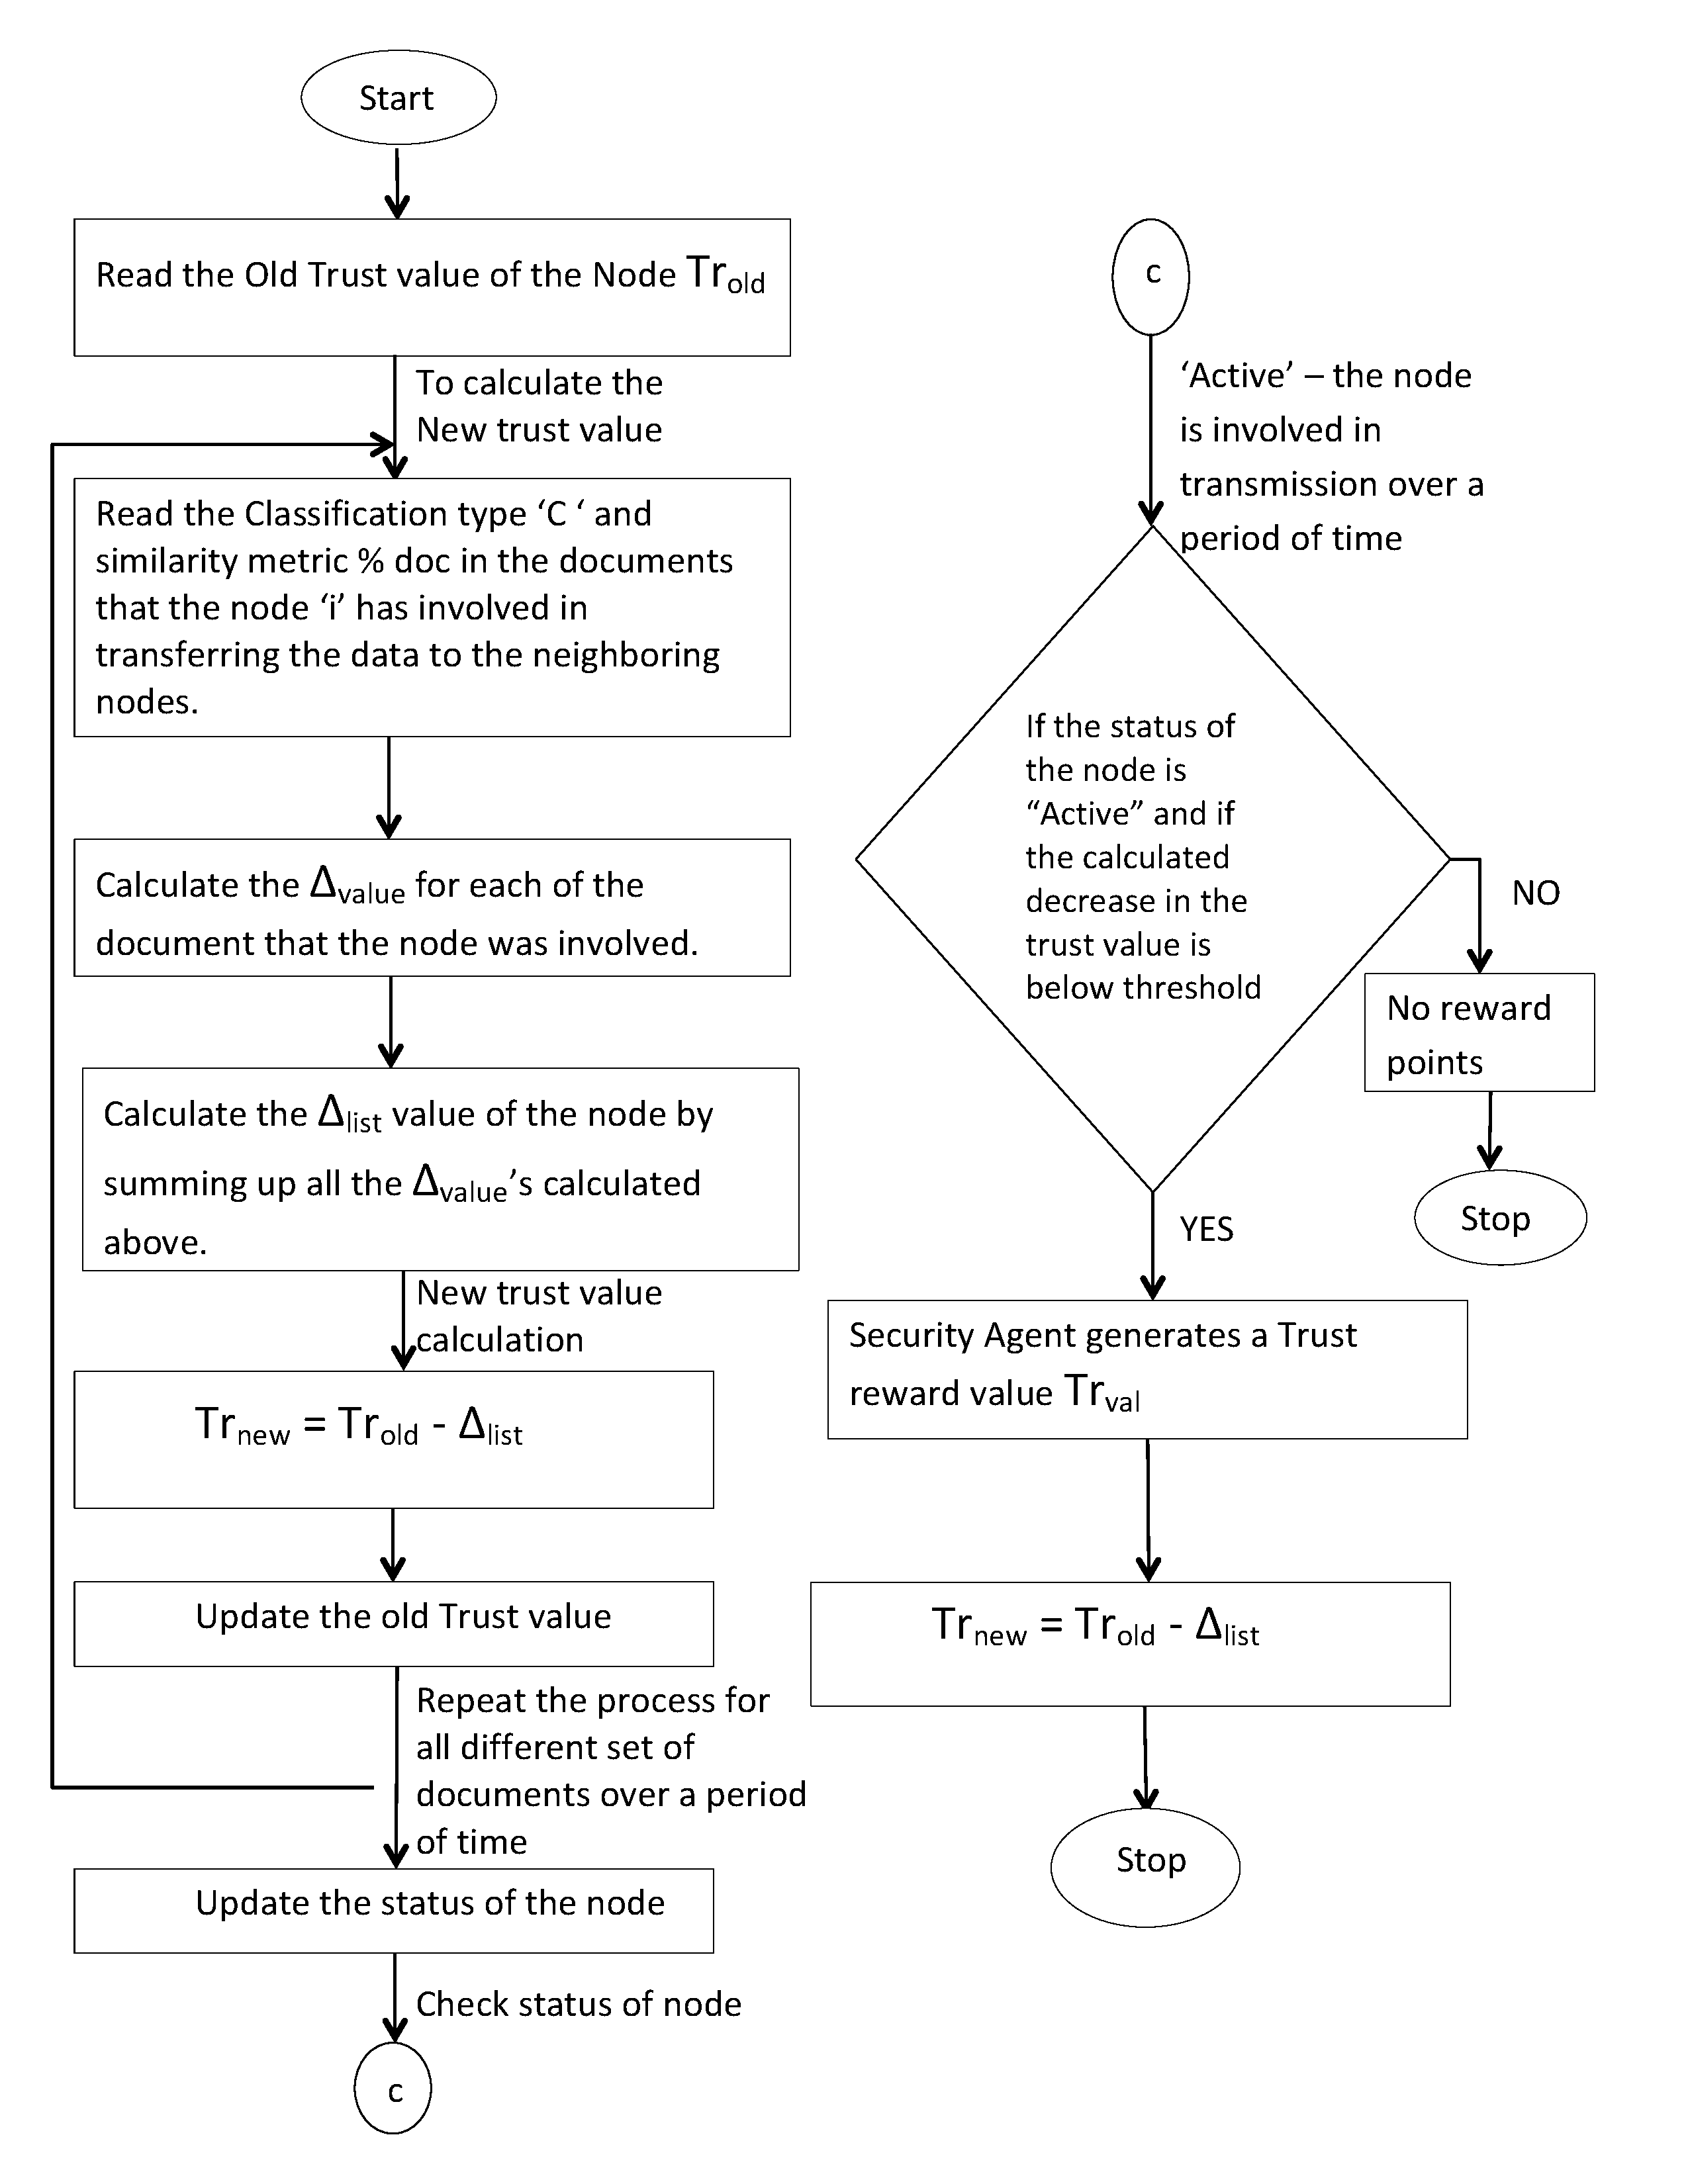
\includegraphics[width=0.90\textwidth]{Figures/Trust_Algorithm.png}
        \caption{Trust Evaluation Algorithm}
    \end{center}
\end{figure}
  
\subsection{Trust Value Testing Results on Various Scenarios}
Table \ref{tab:trust_testing} demonstrates the intermediate steps of calculating
trust. Finally, trust values are updated in Table \ref{tab:trust_evaulation}.
\begin{table}[h!]
    \centering
\begin{tabular}{c | c | c | c | c | c}
    \hline
    Node ID	& DOCUMENT ID	& \( \Delta_{ID} \) 	 & C	& \%doc	& \( \Delta_{value} \) \\
    \hline \hline
1        & 1	&  Doc - 1      & 0.04       & 0.5	& 0.02 \\
1        & 2	&  Doc - 2      & 0.05       & 0.3	& 0.015 \\
1        & 3	&  Doc - 3      & 0.06       & 0.45	& 0.027 \\
\hline
&		&	 	        &            & \textbf{Sum}	& \em{0.062} \\

    \hline
Node ID &	DOCUMENT ID	&  \( \Delta_{ID} \)         & C	& \%doc& \( \Delta_{value} \) \\
\hline \hline
2        &1	  & Doc - 1         & 0.05       & 0.6	& 0.03 \\
2        &2	  & Doc - 2         & 0.08       & 0.8	& 0.064 \\
2        &3	  & Doc - 3         & 0.075      & 0.9	& 0.0675 \\
\hline
&	  &    	            &            & \textbf{Sum}	& 0.\em{1615} \\
    \hline
Node ID &	DOCUMENT ID	&  \( \Delta_{ID} \)         & C	& \%doc	& \(
\Delta_{value} \) \\
\hline \hline
3        &1	  & Doc - 1         & 0.058      & 0.66	& 0.03828 \\
3        &2	  & Doc - 2         & 0.03       & 0.9	& 0.027 \\
3        &3	  & Doc - 3         & 0.095      & 0.2	& 0.019 \\
\hline
& 	  &                 &            & \textbf{Sum}	& \em{0.08428} \\
    \hline
Node ID &	DOCUMENT ID	&  \( \Delta_{ID} \)         & C	& \%doc	 & \(
\Delta_{value} \) \\
\hline \hline
4        &1	  & Doc - 1         & 0.09       & 0.6	& 0.054 \\
4        &2	  & Doc - 2         & 0.045      & 0.44	& 0.0198 \\
4        &3	  & Doc - 3         & 0.095      & 0.77	& 0.07315 \\
\hline
&    &                 &            &	\textbf{Sum}	& \em{0.14695} \\
\end{tabular}

\begin{align*}
    \text{Where}& \\
    C &:= 0 \to 0.1 \\
    D &:= 0 \to 1 \\
    \Delta_{value} &:= C \cdot \%doc
\end{align*}
    \caption{Trust value testing results}
    \label{tab:trust_testing}
\end{table}

\begin{table}[h!]
    \centering
\begin{tabular}{c | c | c | c}
    \hline
    Node ID	& Current Trust Value &	\( \Delta_{List} \) & \( Tr_{new} \)\\
    \hline \hline
1       & 0.45                & 0.062    &    0.388 \\
2       & 0.35                & 0.162    &    0.188 \\
3       & 0.65                & 0.084    &    0.566 \\
4       & 0.5                 & 0.147    &    0.353 \\
\end{tabular}
\caption{Using the results from Table \ref{tab:trust_testing}, trust my be
updated.}
\label{tab:trust_evaulation}
\end{table}
\subsection{Trust Interface to Planning}
\( X \) is a value calculated using the level obtained through classification and the evaluated trust value of a node.
\begin{equation}
    \label{eq:trust_planning_interface}
    \begin{aligned}
        X &= Tr_{new} + \frac{\ln \frac{l}{L}}{10} \\
    \text{Where}~l &:= \text{Node's level} \\
    L &:= \text{Maximum Level}
    \end{aligned}
\end{equation}
The returned value is between 0 and 1 and is sent as an input to the planning phase.
Table 1 where Maximum level = 10 which belongs to the top most employee or node.
\begin{table}[h!]
    \centering
    \begin{tabular}{c | c | c | c}
        \hline
        Node ID	 & \( Tr{new} \) &	Level &	X \\
\hline \hline
1 &	0.388 &	3	 & 0.26760272 \\
2 &	0.188 &	10	 & 0.188 \\
3 &	0.566 &	2	 & 0.405056209 \\
4 &	0.353 &	2	 & 0.192056209 \\
5 &	0.99  &   1	 & 0.759741491 \\
6 &	0.99  &   10 & 	0.99 \\
7 &	0.01  &   10 & 	0.01 \\
8 &	0.5	  &   1	 & 0.269741491 \\
9 &	0.3	  &   2	 & 0.139056209 \\
\end{tabular}
\caption{Test values for Equation~\ref{eq:trust_planning_interface}}
\label{tab:trust_planning}
\end{table}

From Table~\ref{tab:trust_planning}, it is clear that the returned value for
\( X \) is higher for the more trustworthy nodes. Also, if the trust value is same for
two nodes, then the node, which is superior in level, has a slightly larger
value for \( X \).

\subsection{General References}
The following references provided overall general information to this chapter:
\autocite{JiminLi2010}, \autocite{Varadharajan2004},
\autocite{Varadharajan2005}.

